% ****** Start of file aipsamp.tex ******
%
%   This file is part of the AIP files in the AIP distribution for REVTeX 4.
%   Version 4.1 of REVTeX, October 2009
%
%   Copyright (c) 2009 American Institute of Physics.
%
%   See the AIP README file for restrictions and more information.
%
% TeX'ing this file requires that you have AMS-LaTeX 2.0 installed
% as well as the rest of the prerequisites for REVTeX 4.1
% 
% It also requires running BibTeX. The commands are as follows:
%
%  1)  latex  aipsamp
%  2)  bibtex aipsamp
%  3)  latex  aipsamp
%  4)  latex  aipsamp
%
% Use this file as a source of example code for your aip document.
% Use the file aiptemplate.tex as a template for your document.
\documentclass[%
 aip,
% jmp,
% bmf,
% sd,
% rsi,
 amsmath,amssymb,
%preprint,%
 reprint,%
%author-year,%
%author-numerical,%
% Conference Proceedings
]{revtex4-1}
\usepackage{graphicx}% Include figure files
\usepackage{dcolumn}% Align table columns on decimal point
\usepackage{bm}% bold math
%\usepackage[backend=biber]{biblatex}
%\usepackage[mathlines]{lineno}% Enable numbering of text and display math
%\linenumbers\relax % Commence numbering lines
\graphicspath{{Figure/}}
\usepackage[utf8]{inputenc}
\usepackage[T1]{fontenc}
\usepackage{mathptmx}
\usepackage{etoolbox}
\usepackage{microtype}  % Improves spacing globally
%% Apr 2021: AIP requests that the corresponding 
%% email to be moved after the affiliations
\makeatletter
\def\@email#1#2{%
 \endgroup
 \patchcmd{\titleblock@produce}
  {\frontmatter@RRAPformat}
  {\frontmatter@RRAPformat{\produce@RRAP{*#1\href{mailto:#2}{#2}}}\frontmatter@RRAPformat}
  {}{}
}%
\makeatother
\begin{document}

\preprint{AIP/123-QED}

\title[]{Analysis Anomalous Doppler Effect from quantum theory to classical dynamic simulation }
% Force line breaks with \\
\author{A. Author}
 \altaffiliation[Also at ]{Physics Department, XYZ University.}%Lines break automatically or can be forced with \\
\author{B. Author}%
 \email{Second.Author@institution.edu.}
\affiliation{ 
Authors' institution and/or address%\\This line break forced with \textbackslash\textbackslash
}%

\author{C. Author}
 \homepage{http://www.Second.institution.edu/~Charlie.Author.}
\affiliation{%
Second institution and/or address%\\This line break forced% with \\
}%

\date{\today}% It is always \today, today,
             %  but any date may be explicitly specified

\begin{abstract}
A quantum model combined with angular momentum conservation is established to analyze the process of Normal Doppler Effect and Anomalous Doppler Effect, illustrating that the resonance process is related to the angular momentum of the wave. The angular momentum resonant condition is numerically tested, and the energy change ratio between parallel and gyrokinetic energies during electron-wave resonance is calculated, showing strong agreement with quantum theory.
\end{abstract}

\maketitle

%\begin{quotation}
%The ``lead paragraph'' is encapsulated with the \LaTeX\ 
%\verb+quotation+ environment and is formatted as a single paragraph before the first section heading. 
%(The \verb+quotation+ environment reverts to its usual meaning after the first sectioning command.) 
%Note that numbered references are allowed in the lead paragraph.
%%
%The lead paragraph will only be found in an article being prepared for the journal \textit{Chaos}.
%\end{quotation}

\section{\label{sec:level1}INTRODUCTION}

The Anomalous Doppler Effect (ADE)\cite{tamm1959general,frank1960optics,ginzburg1960certain,shustin1971transformation}, in which the observed frequency shift behaves contrary to the conventional Doppler Effect under specific conditions, was first theoretically predicted by Soviet physicist Vitaly L. Ginzburg\cite{ginzburg1946radiation}. This phenomenon occurs when a moving system’s velocity exceeds the phase velocity of light in the medium, it transfers its kinetic energy to its internal energy while emitting radiation. A notable example, discussed by Frank in his 1958 Nobel lecture\cite{frank1960optics}, demonstrates that radiation emission does not result from atomic transitions from a higher (excited) state to a lower state, as is typical, but rather occurs inversely—from a lower state to a higher state—where the energy is supplied by the system’s translational kinetic energy. This intriguing theoretical prediction has attracted significant attention and has motivated extensive research\cite{nezlin1976negative,santini1984anomalous,kho1988slow,wang2016multi,guo2018control,liu2018role,shi2018superlight,filatov2021role}.

In 1967, Artsimovich\cite{artsimovich1967thermal}observed discrepancies in tokamak experiments: measurements of electron temperature derived from diamagnetic signals stronger than derived from electrical conductivity measurement. This anomaly, unrecognized at the time, may represent the first experimental observation of ADE. It was not until 1968 that B. B. Kadomtsev\cite{kadomtsev1968electric}[16]  identified the that cause as ADE, wherein electron’s longitudinal velocity scatter to transverse velocity under resonant ADE conditions. This process amplifies the diamagnetic effect beyond contributions from thermal motion alone. After that, more phenomena related to ADE are observed, such as electron beam scattering in magnetic field vacuum tube[4], wave radiation\cite{spong2018first,liu2019intense,gorozhanin1997waves} [17-19] and runaway electron instability in tokamaks \cite{sajjad2007runaway,castejon2003particle}. Applications based on ADE have also emerged in various areas, such as high-power microwave generation [22] and runaway electron suppression in tokamaks\cite{guo2018control,zhang2024self}.

The physics of the Anomalous Doppler Effect (ADE) was previously explained based on the quantum analysis provided by Frank and Ginzburg\cite{frank1960optics,ginzburg1979nonlinear}. In this paper, building on Ginzburg’s quantum analysis and incorporating angular momentum conservation, we present a more detailed analysis of ADE, offering further insights into the relationship between  wave angular momentum and ADE. Despite the simplicity of the model, to the best of our knowledge, the analysis of angular momentum conservation during the ADE process has not been presented or mentioned before. 

 Additionally, a numerical simulation of a single particle resonating with an electromagnetic (EM) wave in the presence of uniform static electric and magnetic fields is conducted based on classical dynamical equations. This simulation demonstrates the relationship between the wave’s angular momentum and the resonance condition. The energy transfer ratio from the electron's kinetic energy to its gyrokinetic energy during the resonance with the EM wave is computed numerically, and the results show strong agreement with the formula derived from quantum analysis.

The remainder of this paper is organized as follows. Section~\ref{Quantum} presents the quantum analysis based on angular momentum conservation. Section III describes the numerical setup and methodology, including illustrations of the temporal evolution of velocity and kinetic energy. Section IV discusses the energy transfer ratio and polarization characteristics. Finally, Section V provides a brief discussion and conclusion.

\section{Quantum analysis of ADE}\label{Quantum}
We begin with the quantum theory proposed by V.L. Ginzburg\cite{ginzburg2005radiation}based on the energy-momentum conservation, and then incorporate  angular momentum conservation to illustrate the relationship of wave’s angular momentum and Landau level n under the resonant condition $\omega = \vec{k}\cdot \vec{v}+m \omega_{ce}$, where $\omega$ is wave’s angular frequency, $\vec{k}$ represents the wave vector,  $\vec{v}$ means the velocity of electron and $ \omega_{ce}$ is the electron cyclotron angular frequency in static magnetic field, $ m =0,±1,±2,…  $is the quantum number of the Landau levels\cite{coppi1976slide}.

When a charged particle moves through a medium at a speed greater than the phase velocity of light in that medium, it induces polarization in the surrounding molecules. As these molecules return to their equilibrium state, they emit electromagnetic radiation. The constructive interference of these emissions produces the characteristic Cherenkov radiation, forming a cone-shaped wavefront as shown in Fig.~\ref{fig:cherenkov}. The direction of Cherenkov radiation is constrained to the Cherenkov radiation angle $\theta_0 = \arccos\left(\frac{c'}{v}\right)$
,where $ c'$ is the speed of light in the medium and v is the velocity of the charged particles.
\begin{figure}
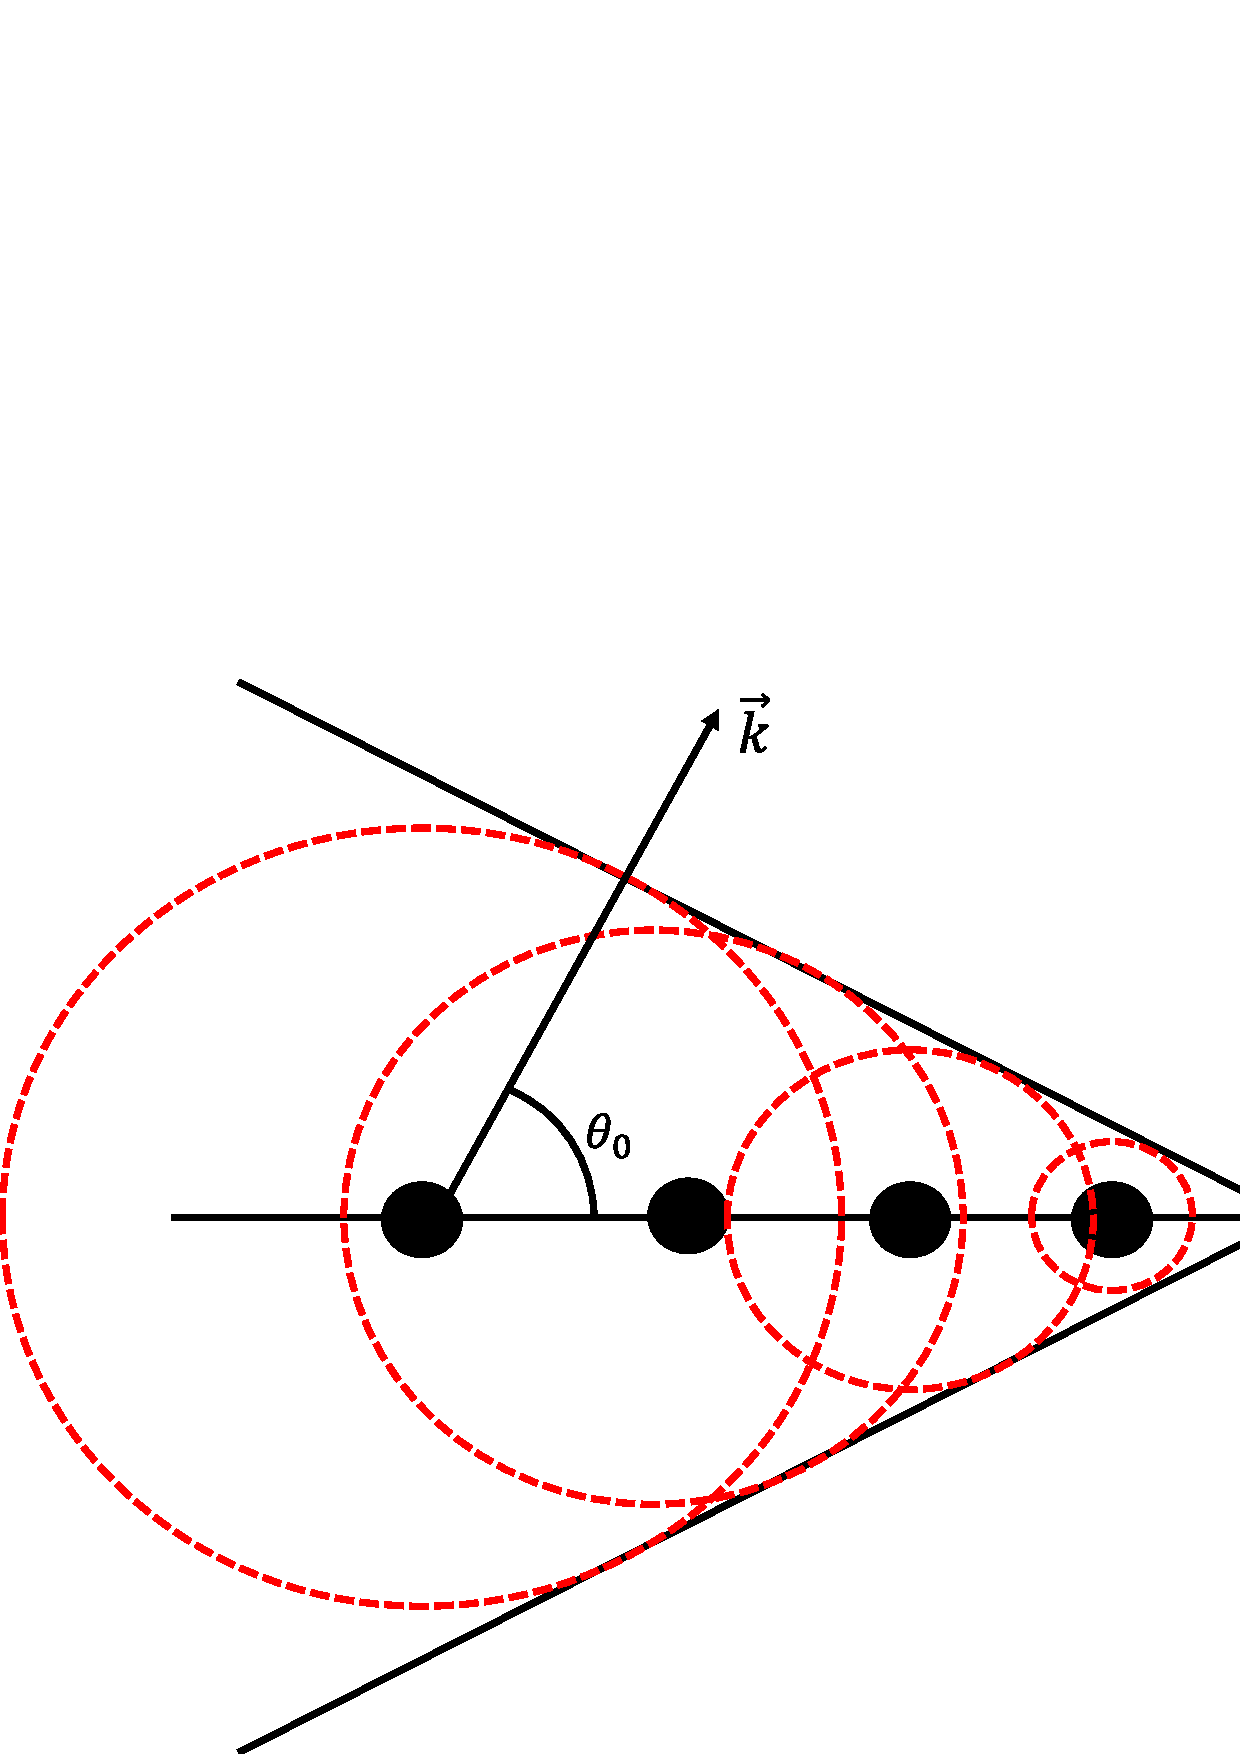
\includegraphics[width=0.4\textwidth]{Figure1.pdf}% Here is how to import EPS art
\caption{\label{fig:cherenkov}Schematic diagram of Cherenkov Radiation. The black points stand for the snapshot of the electron at different times, the read dash circle refers to the current radiation surface from the previous electron.}
\end{figure}

\begin{figure}
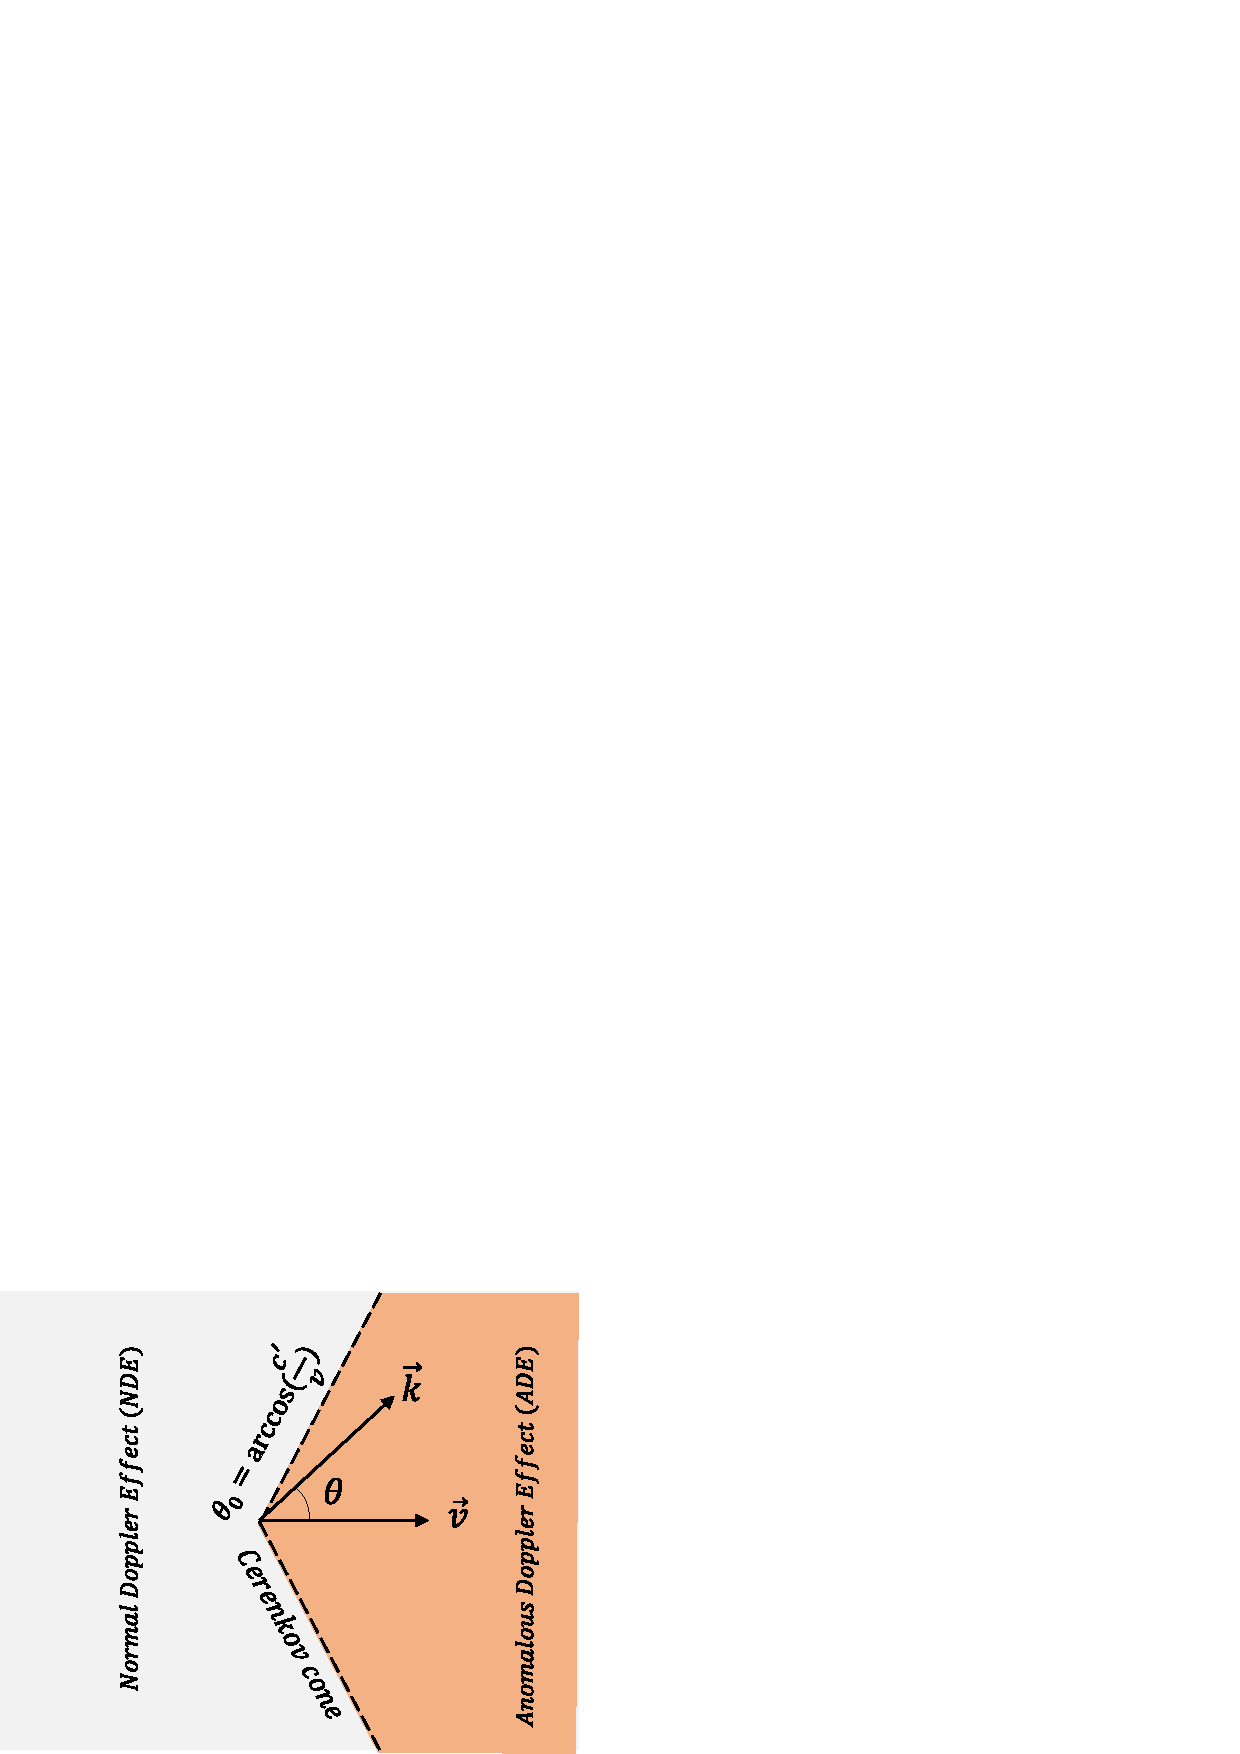
\includegraphics[width=0.4\textwidth]{Figure2.pdf}% Here is how to import EPS art
\caption{\label{fig:ADENDE}The region of Anomalous Doppler Effect (ADE) and Normal Doppler Effect (NDE).}
\end{figure}
However, when the electron is replaced by a system possessing internal energy---such as an oscillator or a cyclotron electron in a magnetic field---the direction of the emitted photon is no longer determined by the interference of secondary waves and can instead occur in any direction. Considering a scenario where the system emits a photon with angular frequency $\omega$ and wavevector k, the emission process must satisfy both energy and momentum conservation:
\begin{subequations}
\begin{eqnarray}
T_1+U_1&=&\hbar \omega +T_2+U_2  \label{Tc} \\  
 \vec{p_1}&=&\vec{p_2}+\hbar\vec{k}   \label{Pc}
\end{eqnarray}
\end{subequations}

Here the T and U represent the kinetic energy and internal energy of the system while subscripts of 1 and 2 refer to before and after emitting a photon. p represents the momentum of the system and $\hbar$ represnts reduced Planck's constant. Assumpting that photon’s energy is far less than the initial kinetic energy $T_1$, the losses of kinetic energy after emitting a photon can be expressed as $\Delta T_{12} = T_1 - T_2 = \Delta\vec{ p} \cdot \vec{v}$, where v is the velocity of the system before emitting a photon and $\Delta\vec{ p} = \vec{p}_1 - \vec{p}_2 = \hbar \vec{k}$. Thus, the change of internal energy can be expressed as 
\begin{equation} 
\begin{array}{rl}
\Delta U_{21} &= \Delta T_{12} - \hbar \omega \\
              &= \hbar \vec{k} \cdot \vec{v} - \hbar \omega \\
              &= \hbar \omega \left( \dfrac{v \cos \theta}{c'} - 1 \right)
\end{array} \label{eq:DeltaU00}
\end{equation}
Here, \(\omega / k = c'\), and \(\Delta U_{21} = U_2 - U_1\). When the system's velocity exceeds the speed of light in the medium (\(v > c'\)), the sign of \(\Delta U_{21}\) allows the radiation to be categorized into three distinct regions, as illustrated in Fig.~\ref{fig:ADENDE}.
\begin{enumerate}
\item For $\theta > \theta_0 = \arccos(c'/v)$, $\Delta U_{21} < 0$. The system produces photons by consuming its own internal and kinetic energy; this region refers to the Normal Doppler Effect (NDE).
\item For $\theta = \theta_0$, $\Delta U_{21} = 0$, the loss of kinetic energy by the system is completely converted into photon energy; this line refers to the Cerenkov Effect.
\item For $\theta < \theta_0$, $\Delta U_{21} > 0$, this region is referred to as the Anomalous Doppler Effect (ADE), where the system gains internal energy after emitting photons. It means the loss of kinetic energy is converted to photons and the system's internal energy.
\end{enumerate}
In previous paper, the change of internal energy is given as $\Delta U = m\hbar\omega_{ce}$, where $m = 0, \pm1, \pm2, \pm3, \ldots$ represent the Landau level, as given by V.\,L. Ginzburg~\cite{ginzburg2005radiation}, Coppi~\cite{coppi1976slide}, Frolov~\cite{frolov1986excitation}, Frank~\cite{frank1960optics}, Tamm~\cite{tamm1959general} and Nezlin~\cite{nezlin1976negative}. The above content revisits the foundational work of V.\,L. Ginzburg~\cite{ginzburg2005radiation}. In the present paper, it is further demonstrated that $m$ actually represents the quantum number associated with the angular momentum of the emitted photon.

Let's consider the process in which an electron cyclotron system under a uniform magnetic field emits a photon, as shown in Fig.~3. The moving electron has the velocity $v_z$ along the background magnetic field and the $v_\perp$ cyclotron velocity. The kinetic energy along $z$ is $T = \gamma m_e c^2 - m_e c^2$, where $\gamma$ refers to the Lorentz factor. The internal energy represents as $U = \frac{1}{2} \gamma m_e v_\perp^2$. 

Assume the angular momentum of the system before and after emitting a photon is $L_1$ and $L_2$, respectively. The angular momentum of photon is $n\hbar$. According to the angular momentum conservation, we have
\begin{equation}
L_1 = L_2 + m\hbar \label{eq:AngularCon} 
\end{equation}

\begin{figure}
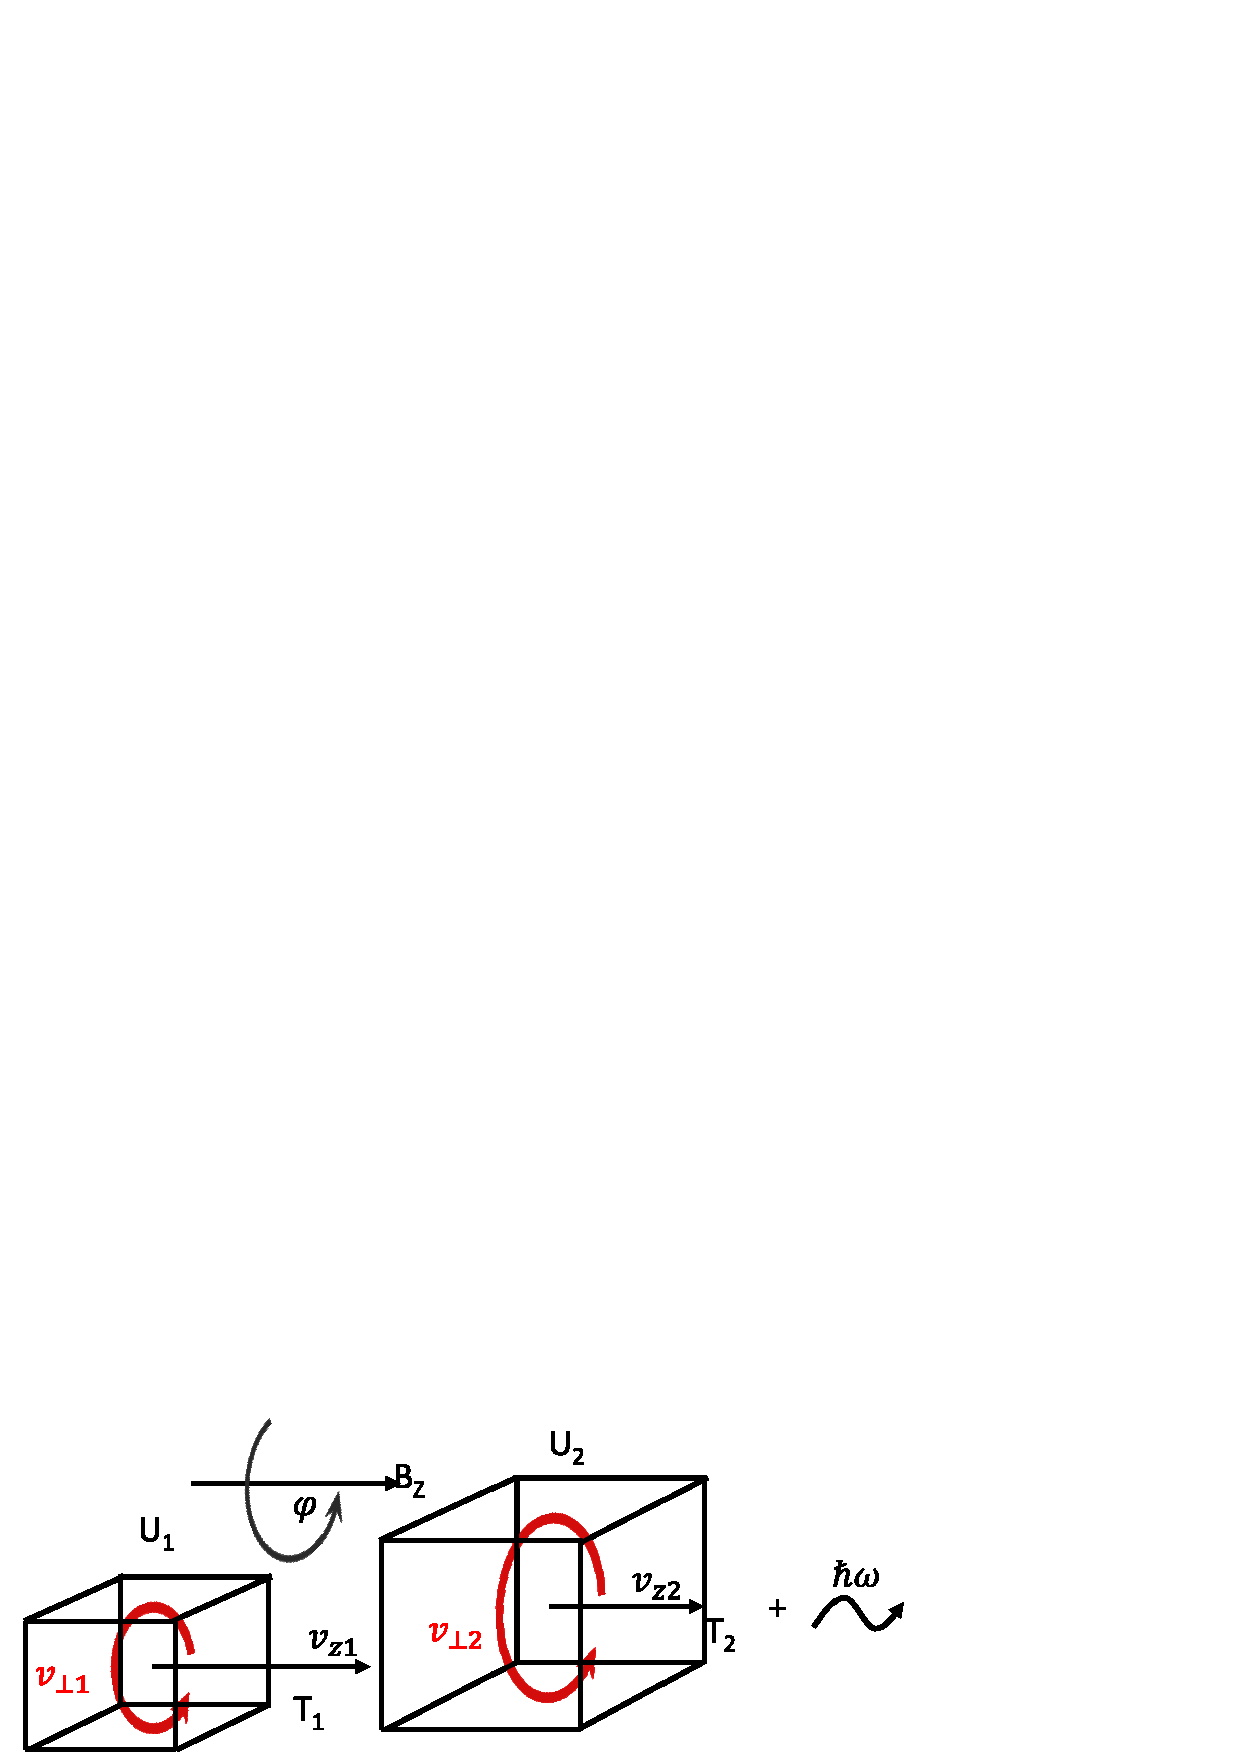
\includegraphics[width=0.5\textwidth]{Figure3.pdf}% Here is how to import EPS art
\caption{\label{fig:Schematic}Schematic diagram of electron cyclotron system before and after emitting a photon. Here \(U2>U1, T2<T1\)}
\end{figure}


Since the magnetic field is aligned along z direction, the angular momentum of electron along z is represented as $L_z$. According to the quantum theory, the electron wave in the static magnetic field can be expressed as
\begin{equation}
\Psi = \Psi_0 e^{\frac{i}{\hbar} (\mathbf{p} - e\mathbf{A}) \cdot \mathbf{s}} \label{eq:psi}
\end{equation}
With the term $\Psi_0$ representing the normalized coefficient, $\mathbf{A}$ is the vector potential and $\mathbf{s}$ is the position. For a gyro-motion electron in a magnetic field, $\mathbf{s} = r\phi\,\vec{e}_\phi$, where $r$ refers to the cyclotron radius and $\phi$ refers to the cyclotron angle. 

The $z$-component of the orbital angular momentum operator can be expressed in spherical coordinates as:
\begin{equation}
\hat{L}_z = -i\hbar\frac{\partial}{\partial\phi} \Psi \label{eq:Lz}
\end{equation}
Combining Eq.~(\ref{eq:psi}) with Eq.~(\ref{eq:Lz}), we have 
\begin{equation}
-i\hbar \frac{\partial}{\partial \phi} \Psi = (p_\phi - eA_\phi) r \Psi
\end{equation}
As a result, the eigenvalue of  $L_z $can be expressed as
\begin{equation}
L_z = (p_\phi - e A_\phi) r  \label{eq:Lz_2}
\end{equation}
With \( p_\phi = \gamma m_e v_\perp \), \( A_\phi = \dfrac{r B_0}{2} \), and \( r = \dfrac{\gamma m_0 v_\perp}{B_0 e} \), Eq.~(\ref{eq:Lz_2}) can be rewritten as:
\begin{equation}
L_z = \frac{1}{2} \cdot \frac{\gamma m_0 v_\perp^2}{\omega_{ce}} = \frac{U}{\omega_{ce}},
\end{equation}
where \(\omega_{ce} = \dfrac{eB}{m_0 \gamma} = \dfrac{\omega_0}{\gamma}\) and \(U = \dfrac{1}{2} \gamma m_0 v_\perp^2\).
Here, \( m_0 \) is the electron rest mass, \( \gamma \) is the Lorentz factor, and \( \omega_0 \) is the electron cyclotron frequency in the rest frame (\( \omega_0 > 0 \)). The conservation of angular momentum in the \( z \)-direction is expressed as
\[
L_{z2} + m\hbar = L_{z1}.
\]
The variation in the angular momentum of the electron along the \( z \)-axis is given by:
\begin{equation}
\Delta L_{21} = L_{z2} - L_{z1} = \frac{U_2 - U_1}{\omega_{ce}} = -m\hbar \label{eq:DeltaL21}
\end{equation}
Here, \( m \) is the quantum number of the photon's angular momentum in the \( z \)-direction. The internal energy change is given by \( \Delta U_{21} = U_2 - U_1 \). With Eq.~(\ref{eq:DeltaL21}), it can be transformed as:
\begin{equation}
\Delta U_{21}=-m \hbar \omega_{ce}  \label{eq:DeltaU21}
\end{equation}
According to the Eq.~(\ref{eq:DeltaU00})  and Eq.~(\ref{eq:DeltaU21}), the change in electron energy  could be presented as 
\begin{equation}
\hbar \vec{k} \cdot \vec{v} = \hbar \omega - m \hbar \omega_{ce}
\end{equation}
This result is consistent with previous findings~\cite{tamm1959general, frank1960optics, nezlin1976negative, coppi1976slide, frolov1986excitation, ginzburg1996radiation}. Here, \( \hbar \vec{k} \cdot \vec{v} \) represents the loss of kinetic energy \( \Delta T_{12} \), \( \hbar \omega \) represents the energy of the photon, and \( -m \hbar \omega_{ce} \) represents the change in the electron gyrokinetic energy \( \Delta U_{21} \) (the internal energy change). The ratio between the internal energy change \( \Delta U_{21} \) and the kinetic energy change \( \Delta T_{12} \) can be expressed as
\begin{equation}
\frac{\Delta U_{21}}{\Delta T_{21}} = \frac{m \hbar \omega_{ce}}{\hbar \vec{k} \cdot \vec{v}}  \label{eq:DU21DT21}
\end{equation}
 This results is a critical criterion to compare with the classical dynamic simulation in the section 2. It is also proved based on classical theory in the Appendix.
After simpifying the Eq.~(\ref{eq:DU21DT21}), we finally have the classical wave-particle resonant condition 
\begin{equation}
\omega = k_z v_z + m \omega_{ce}
\end{equation}
The variable \( m \) represents the quantum number associated with the angular momentum of the photon. Since a photon possesses both orbital angular momentum (\( l\hbar\), where \(l = 0,\pm1,\pm2,\pm3,... \)) and intrinsic spin angular momentum (\( s\hbar \), where \( s = \pm 1 \))~\cite{arnaut2000orbital}, the total angular momentum can be expressed as \( m\hbar = l\hbar + s\hbar \). 

If we consider a plane wave, only the spin angular momentum contributes in this context (i.e., \( l = 0 \)). Therefore, there are two possible scenarios regarding the sign of \( m \), corresponding to the two possible spin states of the photon: \( m = +1 \) or \( m = -1 \).

\begin{enumerate}
\item  	For $m>0$, where $\Delta U_{21}<0$, the internal energy of the cyclotron electron decreases after emitting a photon. If the angular momentum quantum number $m =1$, the emitted photon exhibits right-hand circular polarization. This process is known as the NDE.
\item    	For $m<0, \Delta U_{21}>0$, the cyclotron electron gains internal energy after emitting a photon. The emission photo will have left-hand circular polarization if the angular momentum quantum number $m = -1$. This process is known as the ADE.\footnote{ The difference in the definition of left- and right-hand polarization for m in the paper\cite{kiang2008angular} arises because $\omega_0>0$ is chosen here, where $m>0$ corresponds to the same rotation as the electron's right-hand polarization}
\end{enumerate}


While ADE and NDE describe spontaneous emission phenomena that occur without external field intervention, in our simulation model an external electromagnetic (E.M) waves is introduced as resonant fields interacting with electrons in static magnetic and electric fields. This approach provides a framework for analysing ADE under resonant conditions, referred to here as Anomalous Doppler Resonance (ADR). Under such resonance, both emission and absorption processes can occur, depending on the phase relationship between the electron’s perpendicular velocity and the electric field of the E.M wave. A detailed analysis is provided in the Appendix.


Depsite nonlinear analyses of electron interactions with E.M waves—excluding static electric fields—have been presented in numerous studies \cite{liu2004particle,qian1999exact,weyssow1990motion,gogoberidze2005origin,roberts1964motion,bourdier2000dynamics,nusinovich1999theory,nusinovich1995theory,qian2000relativistic}, fewer investigations have considered the influence of a static electric field during resonance with E.M waves. Due to the complexity of the nonlinear processes involved, analytical solutions are nearly impossible to obtain, making numerical simulations essential in this context.

\section{Classical dynamic simulation of ADR}\label{sec:level2}
The ADE process has been analyzed based on quantum theory, demonstrating that the angular momentum of the emitting photon determines the resonance condition. Specifically, only angular momentum with  $m < 0 $ corresponds to the ADE process, while $m >0 $ corresponds to the NDE process. These characteristics will be tested through the interaction of E.M wave and the electron during ADR and Normal Doppler Resonance (NDR), and the energy transfer ratio can also be verified through numerical simulations.
\subsection{Numerical simulation setup}
To analyze the resonant process from the perspective of classical dynamics and to provide a direct comparison between quantum and classical dynamic results, the following scenario is considered: A uniform magnetic field \( \vec{B}_0 \) is applied along the \( z \)-direction. An electrostatic field \( \vec{E}_0 \), oriented in the opposite direction to \( \vec{B}_0 \) (as illustrated in Fig.~4), is used to accelerate the electron. 

We consider the interaction between an electron entering the system with velocity \( v_z \), parallel to the magnetic field \( B_0 = B_z \), and a linearly or circularly polarized transverse electromagnetic (TEM) wave propagating in a homogeneous dielectric medium with a refractive index \( n > 1 \).

The induced linearly polarized wave along \( \vec{B}_0 \) can be decomposed into a combination of a right-hand circularly polarized wave (\( m = 1 \)) and a left-hand circularly polarized wave (\( m = -1 \)), such that
\(
\vec{E}_w = \vec{E}_R + \vec{E}_L,
\)
where
\(
\vec{E}_R = \frac{1}{2} E_0 (\vec{e}_x + i\vec{e}_y) \exp[i(\vec{k} \cdot \vec{r} - \omega t)],
\vec{E}_L = \frac{1}{2} E_0 (\vec{e}_x - i\vec{e}_y) \exp[i(\vec{k} \cdot \vec{r} - \omega t)].
\)
If the wavevector \( \vec{k} \) lies in the \( y \)-\( z \) plane with a crossing angle \( \theta_k \) relative to the \( z \)-axis, then the new coordinate unit vectors for the wave field expression should be rotated accordingly to align with the direction of \( \vec{k} \). The transformed basis vectors are:
\begin{equation}
\begin{pmatrix}
\vec{e}_x' \\
\vec{e}_y'
\end{pmatrix}
=
\begin{pmatrix}
1 & 0 & 0 \\
0 & \cos\theta_k & \sin\theta_k
\end{pmatrix}
\cdot
\begin{pmatrix}
\vec{e}_x \\
\vec{e}_y \\
\vec{e}_z
\end{pmatrix}
\end{equation}
The magnetic field of E.M wave is
\begin{equation}
\vec{B}_w = \frac{\vec{k} \times \vec{E}_w}{\omega}
\end{equation}

\begin{acknowledgments}
We wish to acknowledge the support of the author community in using
REV\TeX{}, offering suggestions and encouragement, testing new versions,
\dots.
\end{acknowledgments}

\section*{Data Availability Statement}

AIP Publishing believes that all datasets underlying the conclusions of the paper should be available to readers. Authors are encouraged to deposit their datasets in publicly available repositories or present them in the main manuscript. All research articles must include a data availability statement stating where the data can be found. In this section, authors should add the respective statement from the chart below based on the availability of data in their paper.
%
%\begin{center}
%\renewcommand\arraystretch{1.2}
%\begin{tabular}{| >{\raggedright\arraybackslash}p{0.3\linewidth} | >{\raggedright\arraybackslash}p{0.65\linewidth} |}
%\hline
%\textbf{AVAILABILITY OF DATA} & \textbf{STATEMENT OF DATA AVAILABILITY}\\  
%\hline
%Data available on request from the authors
%&
%The data that support the findings of this study are available from the corresponding author upon reasonable request.
%\\\hline
%Data available in article or supplementary material
%&
%The data that support the findings of this study are available within the article [and its supplementary material].
%\\\hline
%Data openly available in a public repository that issues datasets with DOIs
%&
%The data that support the findings of this study are openly available in [repository name] at http://doi.org/[doi], reference number [reference number].
%\\\hline
%Data openly available in a public repository that does not issue DOIs
%&
%The data that support the findings of this study are openly available in [repository name], reference number [reference number].
%\\\hline
%Data sharing not applicable – no new data generated
%&
%Data sharing is not applicable to this article as no new data were created or analyzed in this study.
%\\\hline
%Data generated at a central, large scale facility
%&
%Raw data were generated at the [facility name] large scale facility. Derived data supporting the findings of this study are available from the corresponding author upon reasonable request.
%\\\hline
%Embargo on data due to commercial restrictions
%&
%The data that support the findings will be available in [repository name] at [DOI link] following an embargo from the date of publication to allow for commercialization of research findings.
%\\\hline
%Data available on request due to privacy/ethical restrictions
%&
%The data that support the findings of this study are available on request from the corresponding author. The data are not publicly available due [state restrictions such as privacy or ethical restrictions].
%\\\hline
%Data subject to third party restrictions
%&
%The data that support the findings of this study are available from [third party]. Restrictions apply to the availability of these data, which were used under license for this study. Data are available from the authors upon reasonable request and with the permission of [third party].
%\\\hline
%\end{tabular}
%\end{center}

\appendix

\section{Appendixes}

To start the appendixes, use the \verb+\appendix+ command.
This signals that all following section commands refer to appendixes
instead of regular sections. Therefore, the \verb+\appendix+ command
should be used only once---to set up the section commands to act as
appendixes. Thereafter normal section commands are used. The heading
for a section can be left empty. For example,
\begin{verbatim}
\appendix
\section{}
\end{verbatim}
will produce an appendix heading that says ``APPENDIX A'' and
\begin{verbatim}
\appendix
\section{Background}
\end{verbatim}
will produce an appendix heading that says ``APPENDIX A: BACKGROUND''
(note that the colon is set automatically).

If there is only one appendix, then the letter ``A'' should not
appear. This is suppressed by using the star version of the appendix
command (\verb+\appendix*+ in the place of \verb+\appendix+).

\section{A little more on appendixes}

Observe that this appendix was started by using
\begin{verbatim}
\section{A little more on appendixes}
\end{verbatim}

Note the equation number in an appendix:
\begin{equation}
E=mc^2.
\end{equation}

\subsection{\label{app:subsec}A subsection in an appendix}

You can use a subsection or subsubsection in an appendix. Note the
numbering: we are now in Appendix~\ref{app:subsec}.

\subsubsection{\label{app:subsubsec}A subsubsection in an appendix}
Note the equation numbers in this appendix,produced with the
subequations environment:
\begin{subequations}
\begin{eqnarray}
E&=&mc, \label{appa}
\\
E&=&mc^2, \label{appb}
\\
E&\agt& mc^3. \label{appc}
\end{eqnarray}
\end{subequations}
They turn out to be Eqs.~(\ref{appa}), (\ref{appb}), and (\ref{appc}).

\nocite{*}
\section*{REFERENCE}
\vspace{-2.0em}  
\bibliography{aipsamp_ADE}% Produces the bibliography via BibTeX.
%\addbibresource{aipsamp_ADE.bib}
\end{document}
%
% ****** End of file aipsamp.tex ******